%% ============================================================
%%  SECTION 5 — KỊCH BẢN ĐÁNH GIÁ & KẾT QUẢ  (số liệu: v2)
%% ============================================================
\section{Kịch bản đánh giá và kết quả}
\label{sec:eval}

\subsection{Thiết lập thực nghiệm}

Quy trình đánh giá tuân theo hai tầng phân tách rõ ràng:

\begin{enumerate}[leftmargin=*, itemsep=3pt]
  \item \textbf{Tầng 1 — Ablation studies (Mục~\ref{subsec:abl_fe}--\ref{subsec:abl_outlier}):}
        3 thực nghiệm đối sánh kiểm chứng từng quyết định tiền xử lý \textit{trước} khi chạy
        mô hình chính thức.
        Mục đích: xác nhận bằng số liệu (không chỉ lập luận) rằng các lựa chọn thiết kế
        là đúng đắn.
        Cùng siêu tham số đóng băng, cùng tập Validation, chỉ thay đổi \textbf{một yếu tố} mỗi lần.

  \item \textbf{Tầng 2 — Đánh giá chính thức (Mục~\ref{subsec:main_results}):}
        Sau khi các quyết định pipeline đã được xác nhận ở Tầng 1,
        5 mô hình được huấn luyện và đánh giá trên \textbf{pipeline dứt khoát}.
        \begin{itemize}[itemsep=1pt]
          \item \textbf{Model Selection:} 10-fold Cross-Validation trên Train+Val (85\%).
          \item \textbf{Model Assessment:} đánh giá \textbf{đúng 1 lần} trên Test (15\%)
                — ước lượng không thiên lệch cho hiệu năng thực tế.
        \end{itemize}

  \item \textbf{Tầng 3 — Kiểm toán sau triển khai (Mục~\ref{subsec:audit}):}
        soi hành vi của mô hình đã triển khai trong đúng kịch bản app demo
        (\textit{behavioral testing}); truy vết một hiệu ứng phi lý về tận dữ liệu gốc,
        dẫn tới phát hiện cờ tiện ích chế tác và bản vá mô hình triển khai cuối cùng.
\end{enumerate}

% ─────────────────────────────────────────────────────────────────
\subsection{Thực nghiệm A — Dữ liệu thô vs.\ FE vs.\ FE + PCA}
\label{subsec:abl_fe}

\textbf{Câu hỏi:} Feature Engineering (tách \texttt{city}/\texttt{district} từ địa chỉ)
có thực sự cải thiện mô hình không?
Với bộ dữ liệu chỉ 17 cột gốc, PCA có đáng thêm vào không?

\textbf{Thiết kế:} 4 biến thể đặc trưng $\times$ 3 mô hình đại diện (OLS, Ridge, XGBoost);
siêu tham số đóng băng theo kết quả tinh chỉnh; cùng tập Validation.

\begin{table}[H]
  \centering
  \caption{RMSE Validation theo biến thể đặc trưng — thấp hơn = tốt hơn}
  \label{tab:abl_fe}
  \small
  \begin{tabular}{@{}l c c c@{}}
    \toprule
    \textbf{Biến thể} & \textbf{OLS} & \textbf{Ridge} & \textbf{XGBoost} \\
    \midrule
    V0 — Thô (không FE; mất toàn bộ tín hiệu khu vực) & 2.681 & 2.681 & 1.830 \\
    V1 — FE, không chuẩn hóa                           & 2.586 & 2.586 & 1.657 \\
    \textbf{V2 — FE + chuẩn hóa Z-score}               & \textbf{2.586} & \textbf{2.586} & \textbf{1.657} \\
    V3 — FE + PCA 95\% ($\approx$80 chiều)             & 2.622 & 2.622 & 1.685 \\
    \bottomrule
  \end{tabular}
\end{table}

\begin{figure}[H]
  \centering
  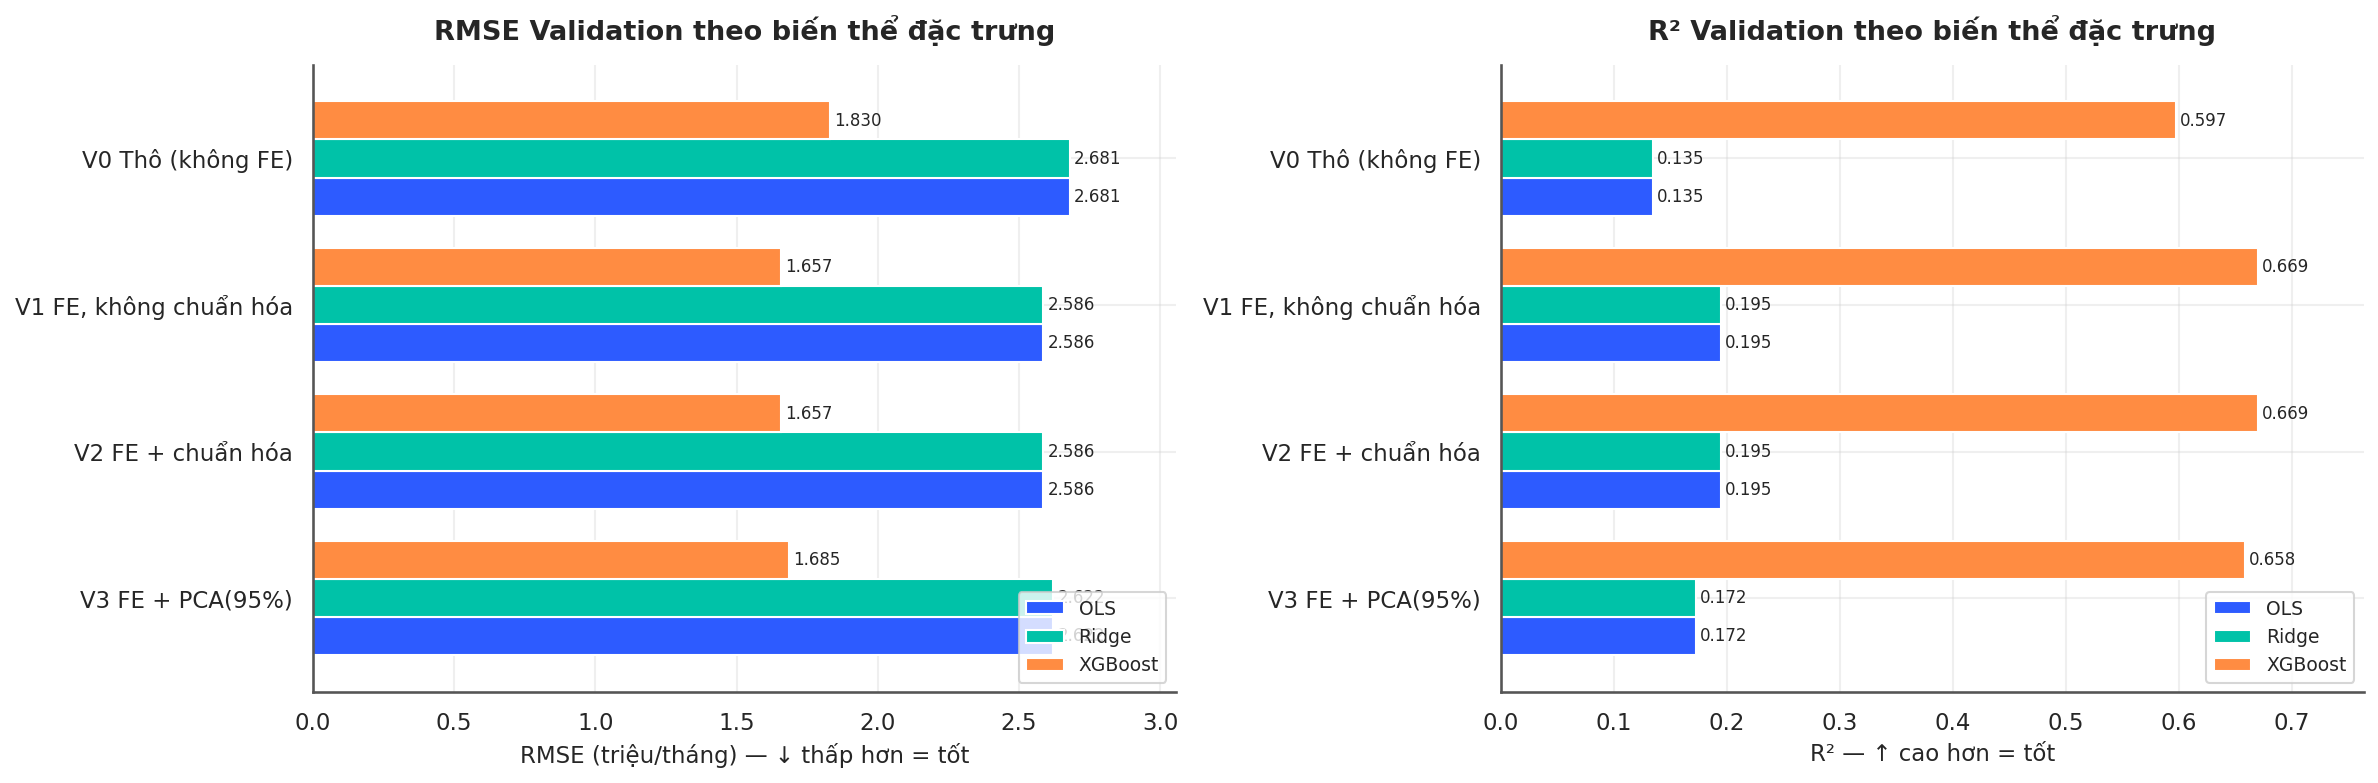
\includegraphics[width=0.90\textwidth]{abl_04_fe_pca}
  \caption{Thực nghiệm A — RMSE và R\textsuperscript{2} theo 4 biến thể đặc trưng.
           FE cải thiện RMSE 3.5\% (tuyến tính) đến 9.4\% (XGBoost) so với dữ liệu thô;
           thêm PCA lại làm tệ hơn 1.4--1.7\%}
  \label{fig:abl_fe}
\end{figure}

\textbf{Kết luận và quyết định:}
{\sloppy
\begin{itemize}[leftmargin=*, itemsep=2pt]
  \item \textbf{Dùng FE (V2):} tách \texttt{city}\slash\texttt{district} từ \texttt{full\_address}
        giảm RMSE \textbf{3.5\% (tuyến tính) đến 9.4\% (XGBoost)} — nguồn cải thiện là
        \textit{mở khóa tín hiệu khu vực} ẩn trong chuỗi địa chỉ (đúng trọng tâm đề tài
        ``theo khu vực'').
  \item \textbf{Không dùng PCA:} $\approx$80 chiều sau One-Hot chưa đủ cao để PCA phát huy;
        nén về $\approx$95\% phương sai loại bỏ mất tín hiệu quận/huyện quan trọng → RMSE tệ hơn.
  \item \textbf{Giữ chuẩn hóa:} không đổi kết quả với OLS/XGBoost
        (bất biến co giãn tuyến tính), nhưng cần thiết cho Ridge/LASSO và PCA.
\end{itemize}
}

\fbox{\textbf{Quyết định A:} Pipeline dứt khoát dùng \textbf{FE + chuẩn hóa Z-score (V2)}.}

% ─────────────────────────────────────────────────────────────────
\subsection[Thực nghiệm B — Biến mục tiêu: price gốc vs. log1p(price)]{Thực nghiệm B — Biến mục tiêu: \texttt{price} gốc vs.\ $\log(1+\text{price})$}
\label{subsec:abl_log}

\textbf{Câu hỏi:} Log-transform biến mục tiêu có thực sự tăng hiệu năng, hay làm mô hình
``underweight'' phân khúc giá cao?
(Giá cao đều có nguyên nhân thực: vị trí trung tâm, đầy đủ tiện ích.)

\textbf{Thiết kế:} ngoài MAE/RMSE/R\textsuperscript{2} toàn cục, đo riêng
\textbf{bias phân khúc giá cao} ($\geq$10 triệu/tháng, 8.3\% Validation):
$\text{bias} = \overline{\hat{y} - y}$; âm nhiều = dự đoán hụt hệ thống.

\begin{table}[H]
  \centering
  \caption{Đối sánh mục tiêu — \texttt{price} gốc vs.\ $\log1p(\text{price})$}
  \label{tab:abl_log}
  \small
  \begin{tabular}{@{}l l r r r r@{}}
    \toprule
    \textbf{Mô hình} & \textbf{Mục tiêu} &
    \textbf{MAE} & \textbf{RMSE} & \textbf{R\textsuperscript{2}} &
    \textbf{Bias giá cao ($\geq$10tr)} \\
    \midrule
    OLS & \textbf{price gốc}  & 1.963 & \textbf{2.586} & \textbf{0.195} & $-5.61$ triệu \\
    OLS & log1p(price) & \textbf{1.882} & 2.636 & 0.164 & $-6.31$ triệu \\
    \addlinespace
    XGBoost & \textbf{price gốc}  & 0.990 & \textbf{1.657} & \textbf{0.669} & $-2.34$ triệu \\
    XGBoost & log1p(price) & \textbf{0.975} & 1.694 & 0.655 & $-2.78$ triệu \\
    \bottomrule
  \end{tabular}
\end{table}

\begin{figure}[H]
  \centering
  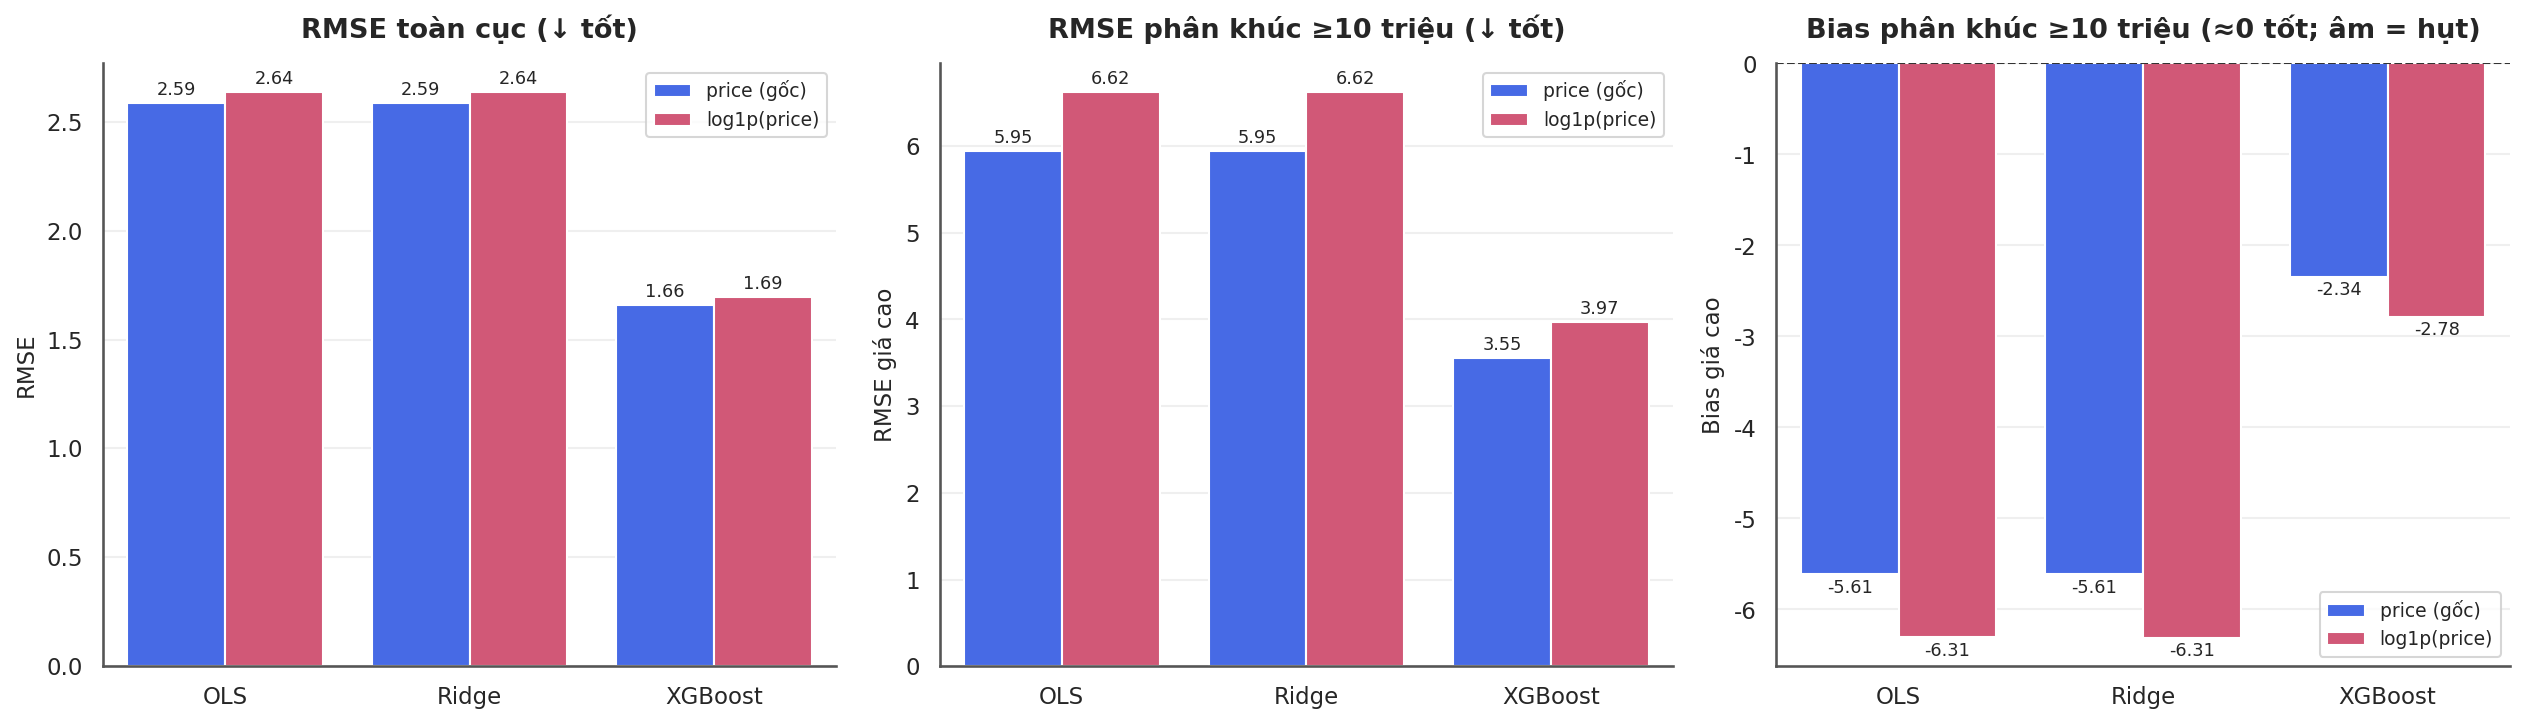
\includegraphics[width=0.90\textwidth]{abl_05_log_target}
  \caption{Thực nghiệm B — RMSE toàn cục (trái), RMSE phân khúc giá cao (giữa),
           Bias giá cao (phải).
           Log chỉ giảm MAE nhẹ; RMSE và bias phân khúc giá cao đều tệ hơn}
  \label{fig:abl_log}
\end{figure}

\textbf{Kết luận và quyết định:}
\begin{itemize}[leftmargin=*, itemsep=2pt]
  \item Log cải thiện MAE $\approx$1.6--4.1\%, nhưng \textbf{RMSE tăng 1.9--2.2\%} và R\textsuperscript{2}
        giảm — không cải thiện theo tiêu chí chọn mô hình chính (RMSE).
  \item \textbf{Bias phân khúc giá cao âm sâu hơn:}
        OLS $-5.61 \to -6.31$ triệu; XGBoost $-2.34 \to -2.78$ triệu.
        Đúng hiện tượng \textit{underweight}: log nén phân khúc giá cao, làm mô hình
        đánh giá thấp các căn hộ đắt dù chúng có nguyên nhân giá thực sự.
  \item Gợi ý log từ phân tích phân phối (EDA) \textbf{bị thực nghiệm bác bỏ}.
\end{itemize}

\fbox{\textbf{Quyết định B:} Cả 5 mô hình huấn luyện trực tiếp trên \textbf{\texttt{price} gốc}.}

% ─────────────────────────────────────────────────────────────────
\subsection{Thực nghiệm C — Tác động của ngoại lệ trong tập huấn luyện}
\label{subsec:abl_outlier}

\textbf{Câu hỏi:} Nếu giữ lại ngoại lệ (giá tới 10.000 triệu $\approx$ 10 tỷ/tháng,
diện tích tới 1.000 m\textsuperscript{2}), hiệu năng trên vùng giá mục tiêu thay đổi thế nào?

\textbf{Thiết kế:} hai mô hình XGBoost hoàn toàn giống nhau, chỉ khác tập Train
(có / không có 6.8\% ngoại lệ);
chấm trên cùng tập Validation vùng mục tiêu (\texttt{price}$\leq$17, \texttt{area}$\leq$180).

\begin{table}[H]
  \centering
  \caption{XGBoost — cùng Validation vùng mục tiêu, chỉ khác tập Train}
  \label{tab:abl_out}
  \begin{tabular}{@{}l c c@{}}
    \toprule
    \textbf{Tập Train} & \textbf{RMSE Validation} & \textbf{So với pipeline chính} \\
    \midrule
    Có ngoại lệ (6.8\% outlier) & 9.747 & $+490\%$ \\
    \textbf{Đã lọc ngoại lệ (pipeline chính)} & \textbf{1.652} & — \\
    \bottomrule
  \end{tabular}
\end{table}

\begin{figure}[H]
  \centering
  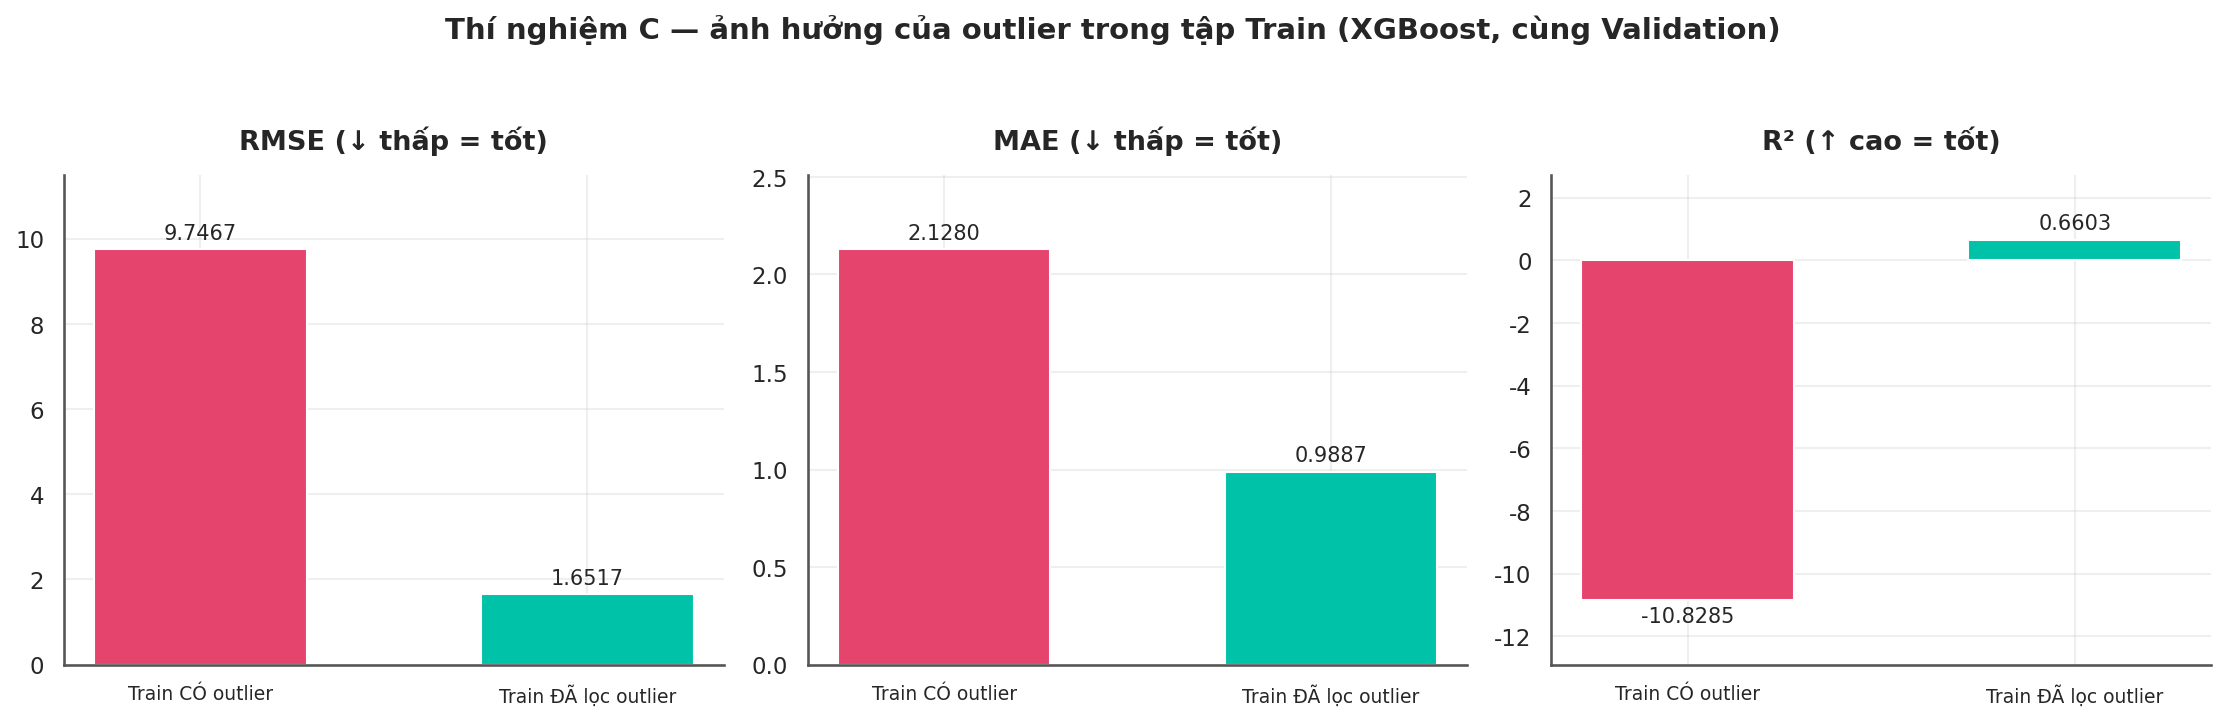
\includegraphics[width=0.90\textwidth]{abl_06_outliers}
  \caption{Thực nghiệm C — RMSE của XGBoost có / không outlier trong Train.
           Giữ outlier làm RMSE xấu hơn $\approx$5.9 lần trên vùng giá mục tiêu}
  \label{fig:abl_out}
\end{figure}

\textbf{Kết luận và quyết định:}
Giữ lại bản ghi giá hàng tỷ/tháng kéo lệch hàm mất mát bình phương —
mô hình phân bổ năng lực học cho vùng giá không bao giờ xuất hiện trong thực tế.
Lọc ngoại lệ giảm RMSE \textbf{83.1\%} trên vùng mục tiêu.

\fbox{\textbf{Quyết định C:} \textbf{Lọc outlier} (\texttt{price}$\leq$17, \texttt{area}$\leq$180) trước khi huấn luyện.}

% ─────────────────────────────────────────────────────────────────
\subsection{Tổng hợp quyết định pipeline}
\label{subsec:pipeline_summary}

Sau 3 thực nghiệm đối sánh, \textbf{pipeline dứt khoát} được xác định:

\begin{table}[H]
  \centering
  \caption{Tổng hợp 3 quyết định thiết kế pipeline — có kiểm chứng thực nghiệm}
  \label{tab:pipeline}
  \begin{tabularx}{\textwidth}{@{}l X l@{}}
    \toprule
    \textbf{Quyết định} & \textbf{Lý do (từ số liệu)} & \textbf{Thực nghiệm} \\
    \midrule
    FE: tách \texttt{city}/\texttt{district} & Giảm RMSE 3.5--9.4\%; PCA không giúp ích & A \\
    Mục tiêu: \texttt{price} gốc & Log tăng RMSE + underweight giá cao & B \\
    Lọc outlier: price$\leq$17, area$\leq$180 & Không lọc làm RMSE $\times$5.9 & C \\
    Mask MNAR + bỏ \texttt{n\_features} + ràng buộc đơn điệu &
      7/12 cờ tiện ích chế tác; hiệu ứng tiện ích âm phi lý & D (Mục~\ref{subsec:audit}) \\
    \bottomrule
  \end{tabularx}
\end{table}

\textbf{Kết quả ở Mục~\ref{subsec:main_results} dưới đây được tính trên pipeline sau
quyết định A--C} (so sánh họ mô hình và chọn mô hình triển khai); quyết định D đến từ
kiểm toán \textit{sau} bước này và chỉ áp dụng cho mô hình triển khai
(Mục~\ref{subsec:audit}).

% ─────────────────────────────────────────────────────────────────
\subsection{Kết quả chính: 10-fold CV và đánh giá Test}
\label{subsec:main_results}

5 mô hình được huấn luyện và đánh giá với \textbf{pipeline đã được xác nhận} ở Mục~\ref{subsec:pipeline_summary}:
dùng FE (city/district), mục tiêu \texttt{price} gốc, dữ liệu đã lọc ngoại lệ.

\begin{table}[H]
  \centering
  \caption{So sánh 5 mô hình — 10-fold CV (Train+Val) và đánh giá Test 1 lần duy nhất.
           $\star$ = mô hình triển khai.}
  \label{tab:model_compare}
  \begin{tabular}{@{}l r@{$\;\pm\;$}l r r r r@{}}
    \toprule
    \textbf{Mô hình} &
    \multicolumn{2}{c}{\textbf{CV RMSE}} &
    \textbf{CV R\textsuperscript{2}} &
    \textbf{Test MAE} & \textbf{Test RMSE} & \textbf{Test R\textsuperscript{2}} \\
    \midrule
    OLS           & 2.582 & 0.018 & 0.193 & 1.958 & 2.586 & 0.190 \\
    Ridge         & 2.582 & 0.018 & 0.193 & 1.958 & 2.586 & 0.190 \\
    LASSO         & 2.587 & 0.019 & 0.190 & 1.961 & 2.589 & 0.188 \\
    Random Forest & \textbf{1.657} & 0.012 & \textbf{0.668} & \textbf{1.002} & \textbf{1.666} & \textbf{0.664} \\
    \midrule
    \textbf{XGBoost} $\star$
      & 1.881 & 0.008 & 0.572 & 1.257 & 1.895 & 0.565 \\
    \bottomrule
  \end{tabular}
\end{table}

\begin{figure}[H]
  \centering
  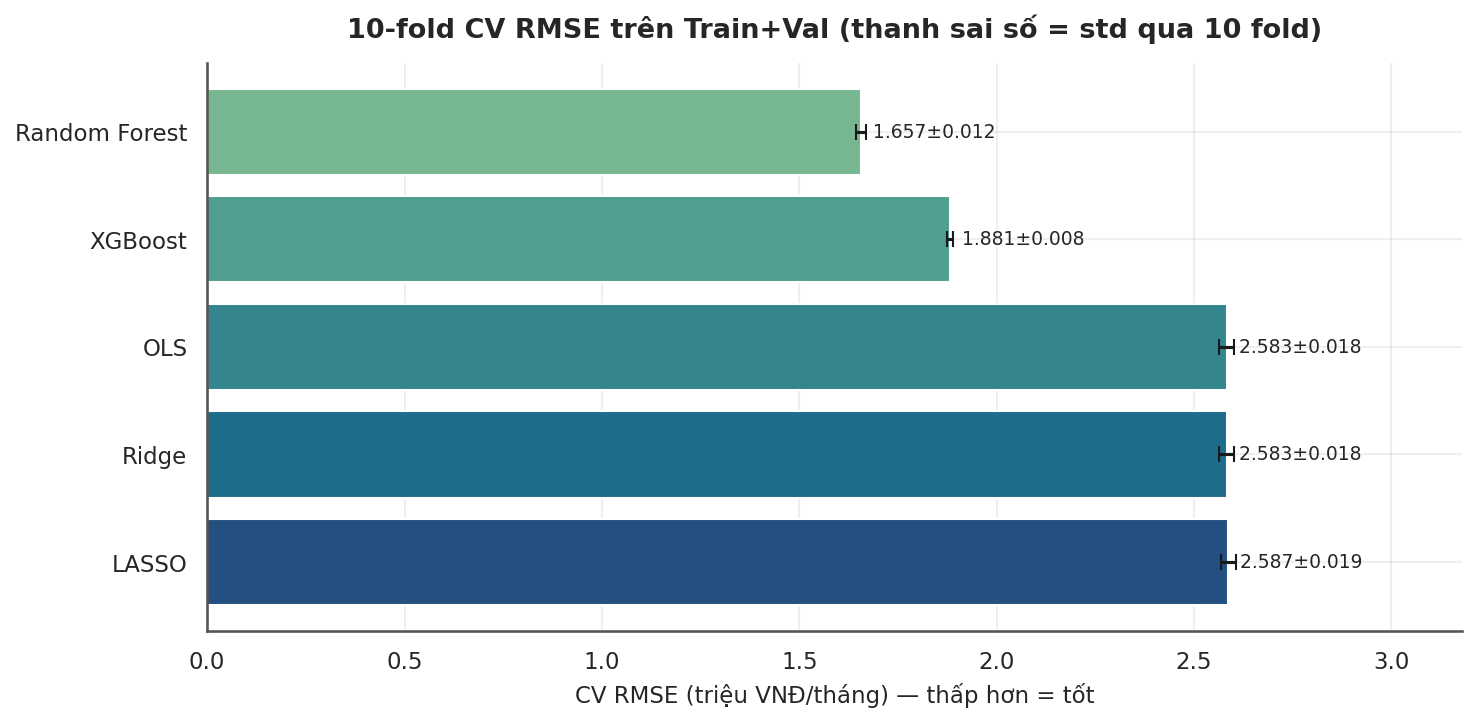
\includegraphics[width=0.86\textwidth]{eval_01_cv_rmse_comparison}
  \caption{CV RMSE của 5 mô hình (mean $\pm$ std, 10 fold) —
           mô hình cây vượt trội (RF $\approx$1.66, XGBoost $\approx$1.88 vs.\ $\approx$2.58 của
           tuyến tính); std nhỏ xác nhận ổn định qua các cách chia}
  \label{fig:cv_compare}
\end{figure}

\begin{figure}[H]
  \centering
  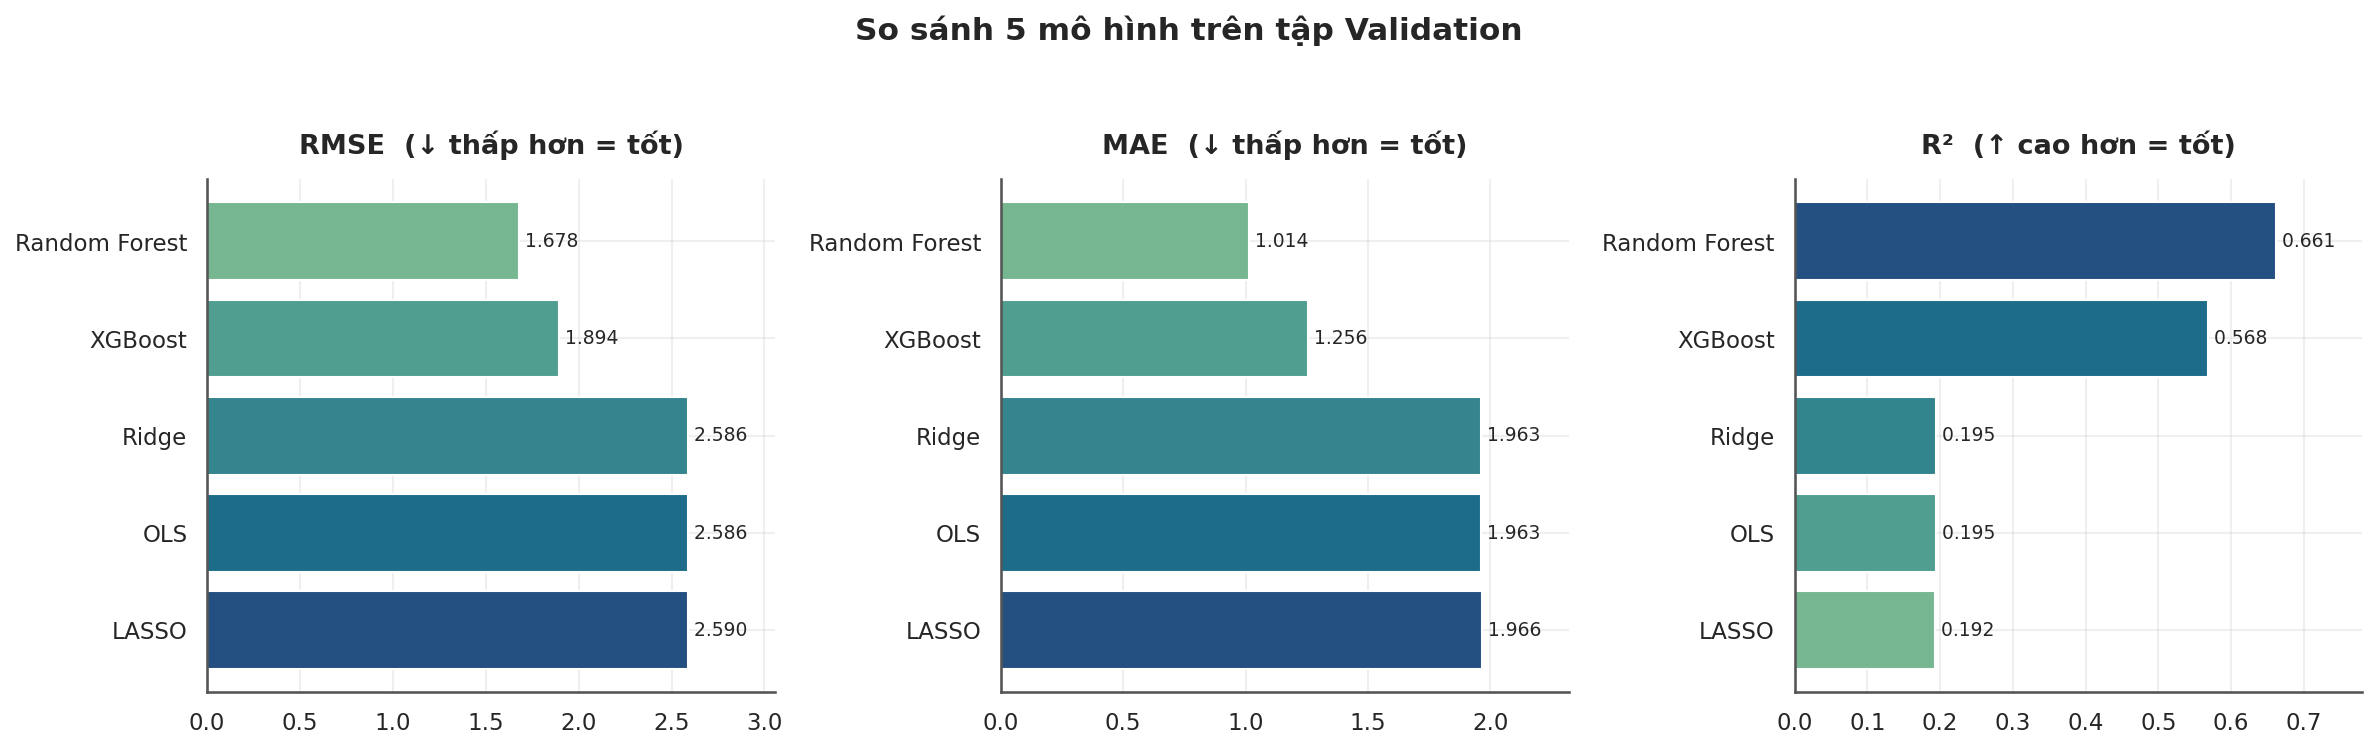
\includegraphics[width=0.86\textwidth]{model_01_model_comparison_val}
  \caption{So sánh RMSE, MAE và R\textsuperscript{2} trên tập Validation — hai mô hình cây
           cách xa tuyến tính; Random Forest nhỉnh hơn XGBoost (XGBoost có ràng buộc đơn điệu
           nên đánh đổi một phần chỉ số lấy hành vi đúng — Mục~\ref{subsec:audit})}
  \label{fig:val_compare}
\end{figure}

\textbf{Phân tích kết quả:}
\begin{itemize}[leftmargin=*, itemsep=3pt]
  \item Mô hình cây \textbf{vượt trội rõ rệt} so với tuyến tính
        (Test R\textsuperscript{2}: $\approx$0.57--0.66 vs.\ $\approx$0.19),
        xác nhận quan hệ phi tuyến và tương tác khu vực $\times$ diện tích
        được gợi ý từ PCA ở Mục~\ref{subsec:clustering}.
  \item CV RMSE $\approx$ Test RMSE, std nhỏ $\Rightarrow$ mô hình \textbf{không overfit},
        khái quát hóa tốt.
  \item \textbf{Chính xác nhất là Random Forest} (Test R\textsuperscript{2} = 0.664), nhưng
        \textbf{mô hình triển khai là XGBoost} (Test R\textsuperscript{2} = 0.565) vì hai lý do
        \textit{vượt trên chỉ số thô}:
        \begin{enumerate}[leftmargin=1.2em, itemsep=1pt, topsep=2pt]
          \item \textbf{Hành vi đúng cho app:} XGBoost mang \textbf{ràng buộc đơn điệu} đảm bảo
                tick thêm tiện ích không làm giảm giá (Mục~\ref{subsec:audit}); Random Forest ở
                đây chạy \textit{không ràng buộc}, nên một phần độ chính xác của nó đến từ tự do
                khai thác tương quan hành-vi-đăng-tin phi nhân quả — sai với người dùng app.
          \item \textbf{Triển khai được:} XGBoost $\approx$0.86 MB so với Random Forest $\approx$5.6 MB
                ($n=200$ cây), nạp/suy luận nhanh hơn trong app, lại có early stopping.
        \end{enumerate}
        Khoảng cách 0.664 vs.\ 0.565 chính là \textbf{cái giá có chủ đích} của việc từ chối
        tương quan phi nhân quả (phân tích kỹ ở Mục~\ref{subsec:audit}).
\end{itemize}

% ─────────────────────────────────────────────────────────────────
\subsection{Biểu đồ chẩn đoán mô hình triển khai (XGBoost)}
\label{subsec:diagnostics}

\begin{figure}[H]
  \centering
  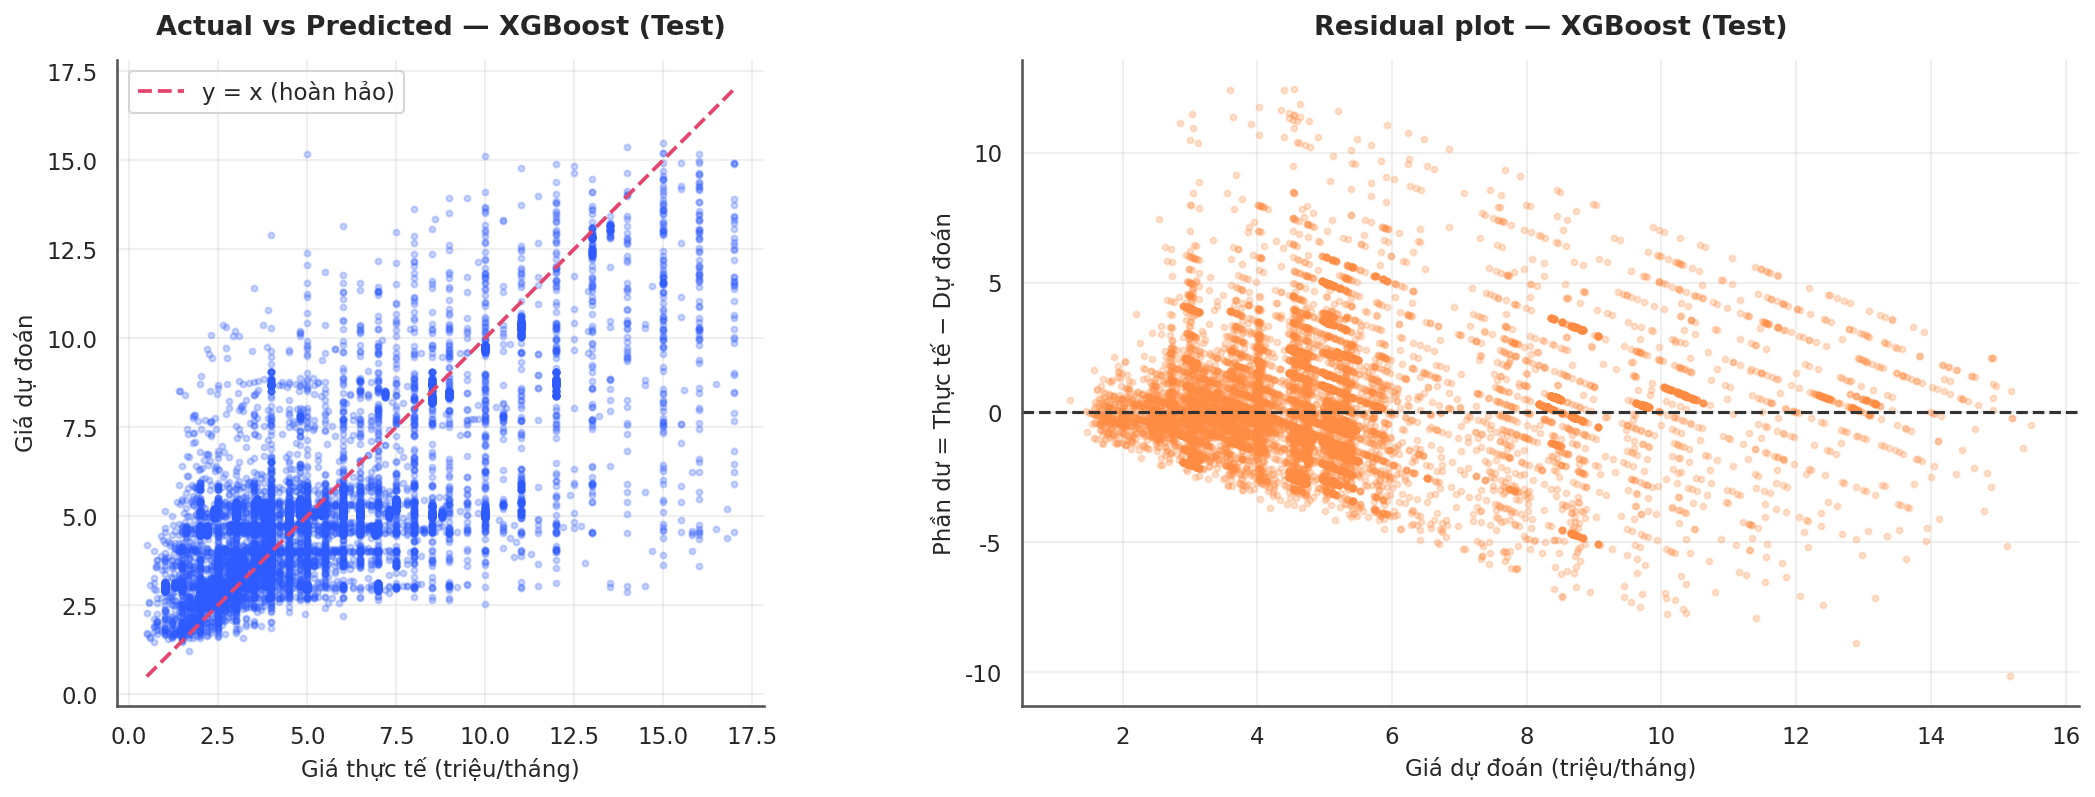
\includegraphics[width=0.86\textwidth]{eval_02_test_actual_vs_pred}
  \caption{Test — Actual vs Predicted (trái) và Residual vs Predicted (phải).
           Điểm bám sát đường $y=x$; phần dư phân tán quanh 0 (mean $\approx$0)
           $\Rightarrow$ không thiên lệch hệ thống}
  \label{fig:test_pred}
\end{figure}

\begin{figure}[H]
  \centering
  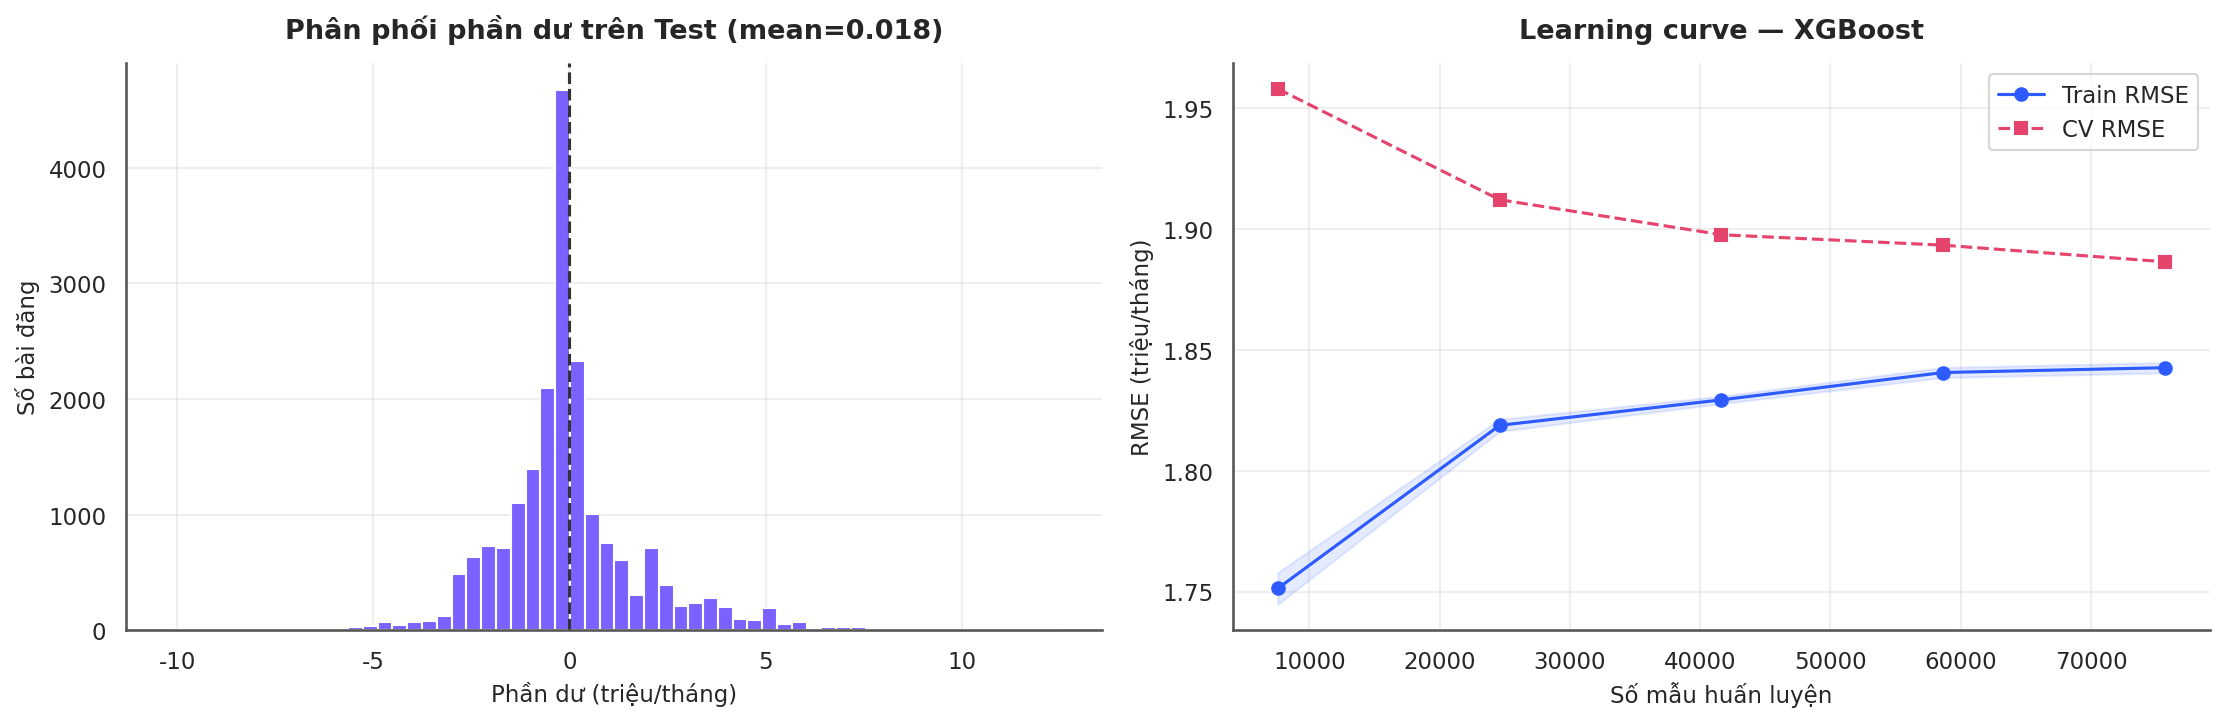
\includegraphics[width=0.86\textwidth]{eval_03_residual_learning_curve}
  \caption{Phân phối phần dư (trái) và Learning curve (phải).
           Train RMSE và CV RMSE hội tụ khi tăng dữ liệu $\Rightarrow$ không overfit nặng;
           khoảng cách còn lại là \textit{bias} — cần đặc trưng mới (GPS, NLP mô tả)}
  \label{fig:lc}
\end{figure}

\begin{figure}[H]
  \centering
  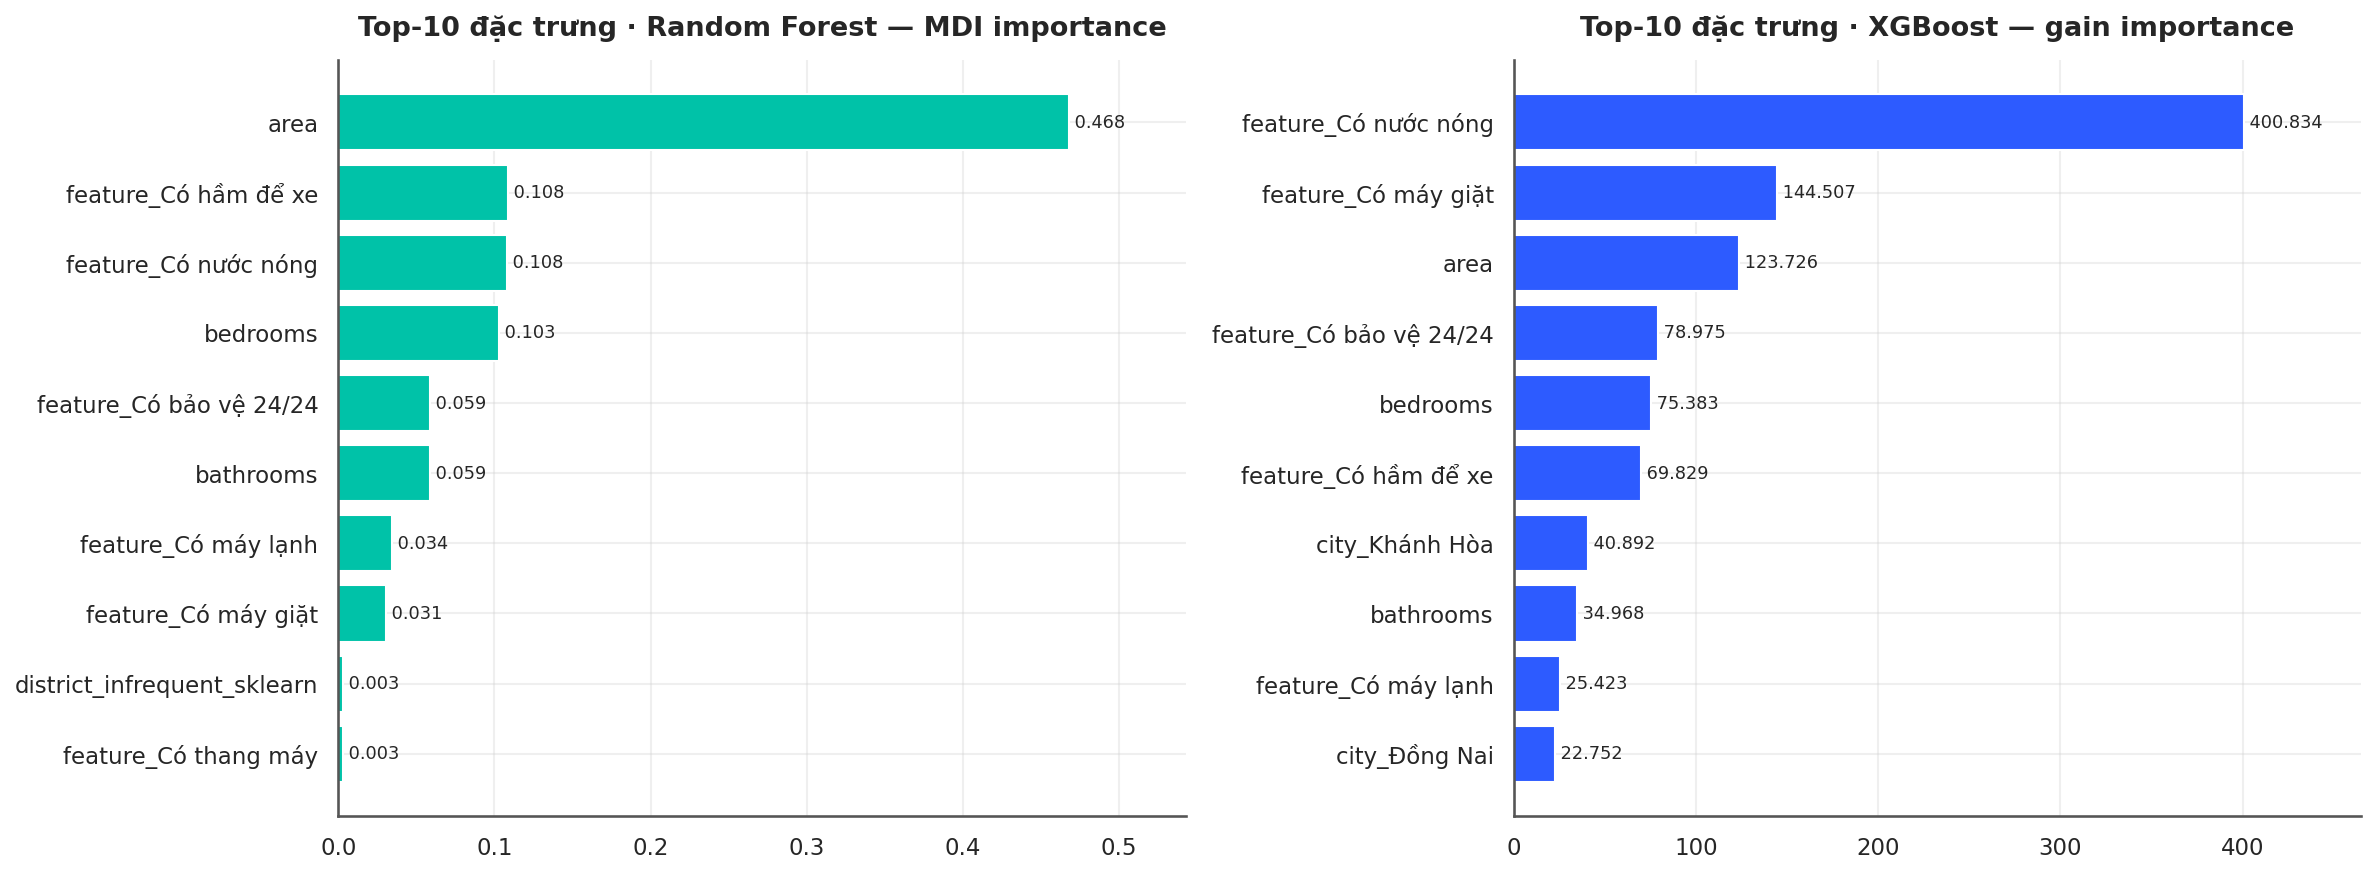
\includegraphics[width=0.84\textwidth]{model_02_feature_importance}
  \caption{Feature Importance — RF (MDI, trái) và XGBoost (gain, phải).
           Sau khi loại \texttt{source}, đặc trưng dẫn đầu là \texttt{area} và
           tiện ích/khu vực — đúng yếu tố định giá thực tế,
           xác nhận giá trị của FE (Thực nghiệm A)}
  \label{fig:importance}
\end{figure}

% ─────────────────────────────────────────────────────────────────
\subsection{Thực nghiệm D — Kiểm toán sau triển khai: cờ tiện ích chế tác
            (MNAR) và ràng buộc đơn điệu}
\label{subsec:audit}

\subsubsection*{Hiện tượng kích hoạt: kiểm thử hành vi trên app demo}

Chỉ số tổng hợp (RMSE/R\textsuperscript{2}) không nói hết về một mô hình.
Khi kiểm thử app demo với input điển hình (25 m\textsuperscript{2}, 1 phòng ngủ,
1 phòng tắm, Hà Nội), việc \textbf{tick ``Có máy lạnh'' làm giá dự báo GIẢM 0.34
triệu/tháng} — phi lý về kinh tế học. Phân rã hiệu ứng cho thấy ngoài máy lạnh
($-0.34$), ba tiện ích khác cũng mang hiệu ứng âm (máy giặt $-0.42$, nước nóng $-0.27$,
hầm để xe $-0.17$), và đường ``tick dần 12 tiện ích''
\textbf{không đơn điệu} (vi phạm 7 lần).

\subsubsection*{Điều tra nguyên nhân: dấu vân tay nguồn}

Phân tích phân tầng chỉ ra cơ chế: nguồn \texttt{nhatot} là phân khúc đắt
(trung vị \textbf{9.0} triệu so với $\approx$4.0 triệu của các nguồn khác) nhưng tỷ lệ
bật cờ tiện ích thấp bất thường (máy lạnh 22\% so với 67--75\% nơi khác; máy giặt 11\%;
nước nóng 6\%). Hệ quả là nhóm ``máy lạnh = 0'' chứa 18.7\% tin \texttt{nhatot}, còn nhóm
``máy lạnh = 1'' chỉ 2.4\% — vì \texttt{source} đã bị loại (đúng đắn, Mục~\ref{subsec:simpson}),
mô hình dùng \textit{pattern cờ tiện ích như dấu vân tay nguồn}: ``không tick máy lạnh
$\Rightarrow$ giống tin nhatot $\Rightarrow$ đắt''. Trong khi đó, hiệu ứng thật của máy lạnh
\textit{trong từng nguồn} và trong đúng phân khúc app dự báo (Hà Nội, 20--30 m\textsuperscript{2})
là $\approx 0$ đến $+0.2$ triệu.

\subsubsection*{Kiểm toán nguồn gốc dữ liệu: 7/12 cờ bị chế tác}

Truy ngược về dữ liệu thô của từng nguồn (đối chiếu tỷ lệ bật cờ
raw $\leftrightarrow$ sau hợp nhất) phát hiện vấn đề nghiêm trọng hơn:

\begin{table}[H]
  \centering
  \caption{Kiểm toán nguồn gốc 12 cờ tiện ích: cờ có cột gốc thật theo nguồn}
  \label{tab:audit_flags}
  \small
  \begin{tabularx}{\textwidth}{@{}L{4.6cm} C{2.2cm} X@{}}
    \toprule
    \textbf{Nguồn} & \textbf{Số cờ thật} & \textbf{Ghi chú} \\
    \midrule
    chothuephongtro, nhatot,\newline facebook, github\_housing & 5/12 &
      máy lạnh, máy giặt, nước nóng, bảo vệ 24/24, hầm để xe
      (tỷ lệ raw $\leftrightarrow$ hợp nhất khớp tới $\approx$1\%) \\
    lozido & 10/12 & thêm gác, kệ bếp, thang máy, không chung chủ, giờ giấc \\
    phongtro123 & 11/12 & thiếu duy nhất nước nóng \\
    chothuenhadattoanvn,\newline github\_hcm/hn/dn ($\approx$16.6\% dữ liệu) & \textbf{0/12} &
      dữ liệu thô không có cột tiện ích nào \\
    \bottomrule
  \end{tabularx}
\end{table}

Bảy cờ còn lại (tủ lạnh, nội thất, gác, kệ bếp, thang máy, không chung chủ, giờ giấc)
chỉ tồn tại thật ở \texttt{phongtro123} + \texttt{lozido} ($\approx$3\% dữ liệu);
với các nguồn khác chúng được \textbf{điền ngẫu nhiên ở bước tích hợp} —
bằng chứng thống kê: tương quan với giá \textit{trong từng nguồn} của các ô chế tác
$\leq 0.013$ (bằng 0 tuyệt đối, đặc trưng của biến ngẫu nhiên độc lập).
Đây cũng chính là lời giải cho các tương quan ``chết'' ở Bảng~\ref{tab:simpson}.

\subsubsection*{Bản vá ba lớp và kết quả}

\begin{enumerate}[leftmargin=*, itemsep=2pt]
  \item \textbf{Mask MNAR:} ô (nguồn, cờ) chế tác $\to$ NaN — ``không khai báo''
        $\neq$ ``không có''. XGBoost xử lý NaN trực tiếp (học nhánh riêng cho
        ``không khai báo''); lúc dự đoán, người dùng app khai báo trực tiếp nên kênh
        NaN không bao giờ kích hoạt.
  \item \textbf{Loại \texttt{n\_features}:} tổng của 12 cờ trong đó 7 cờ là số giả.
  \item \textbf{Ràng buộc đơn điệu} (+1 cho 12 cờ, Mục~\ref{sec:method}): cần thiết vì
        sau khi làm sạch số giả, dữ liệu vẫn còn confound \textit{thật} về hành vi
        đăng tin — phòng giá rẻ quảng cáo tiện ích, căn hộ đắt không liệt kê —
        khiến mô hình chỉ-mask vẫn còn \textbf{7/12 cờ tiện ích mang hiệu ứng âm}
        (Bảng~\ref{tab:audit_results}). XGBoost được search \textit{kèm ràng buộc ngay từ
        đầu} (cấu hình chọn: depth 10, lr 0.05, 126 cây — Mục~\ref{sec:method}).
        Ràng buộc thêm cho \texttt{area} đã được cân nhắc nhưng \textbf{loại} vì làm sập
        độ chính xác (quan hệ \texttt{area}--giá không hoàn toàn đơn điệu cục bộ trong dữ liệu).
\end{enumerate}

\begin{table}[H]
  \centering
  \caption{Thực nghiệm D — ba biến thể trên cùng tập Test. ``Cờ âm'' = số tiện ích
           làm giảm giá khi tick trên app; ``Vi phạm đơn điệu'' = số lần giảm giá khi tick dần
           12 tiện ích. $\star$ = mô hình triển khai cuối.}
  \label{tab:audit_results}
  \small
  \begin{tabular}{@{}l r r r c c@{}}
    \toprule
    \textbf{Biến thể} & \textbf{Test MAE} & \textbf{Test RMSE} &
    \textbf{Test R\textsuperscript{2}} & \textbf{Cờ âm} & \textbf{Vi phạm đơn điệu} \\
    \midrule
    Ban đầu (cờ thô, có \texttt{n\_features})    & 1.072 & 1.740 & 0.633 & 4 & 7 \\
    Chỉ mask MNAR (không ràng buộc)              & \textbf{0.984} & \textbf{1.647} & \textbf{0.671} & 7 & 4 \\
    \textbf{Mask + ràng buộc đơn điệu} $\star$   & 1.257 & 1.895 & 0.565 & \textbf{0} & \textbf{0} \\
    \bottomrule
  \end{tabular}
\end{table}

\begin{figure}[H]
  \centering
  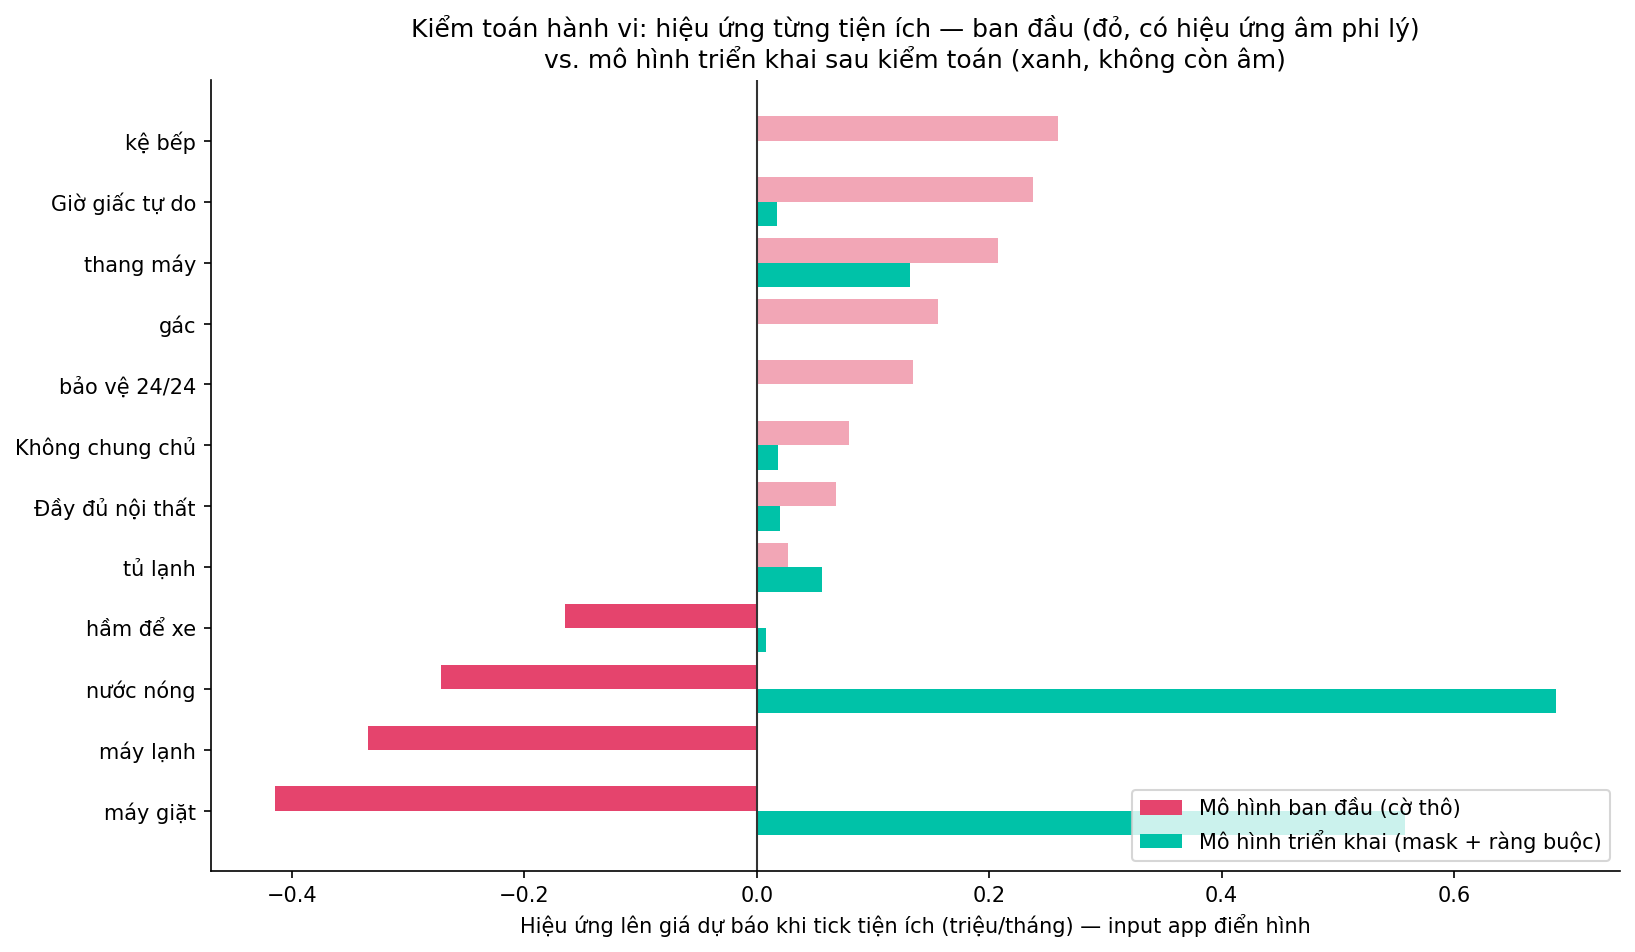
\includegraphics[width=0.92\textwidth]{audit_amenity_effects}
  \caption{Hiệu ứng tick từng tiện ích lên giá dự báo (input app điển hình) —
           mô hình ban đầu có 4 hiệu ứng âm phi lý (đỏ);
           mô hình triển khai sau kiểm toán không còn hiệu ứng âm nào (xanh)}
  \label{fig:audit_effects}
\end{figure}

\textbf{Phân tích đánh đổi — phần thảo luận quan trọng nhất của đồ án:}
\begin{itemize}[leftmargin=*, itemsep=3pt]
  \item \textbf{Làm sạch số giả tự nó cải thiện độ chính xác} (R\textsuperscript{2}
        $0.633 \to 0.671$ — thậm chí cao hơn cả Random Forest 0.664): các cờ chế tác là
        nhiễu kéo mô hình xuống. Điều này cũng cho thấy con số 0.633 ban đầu được ``bơm''
        một phần bởi trò nhận diện nguồn qua pattern cờ — không phải tín hiệu định giá thật.
  \item \textbf{Khoảng cách $0.671 \to 0.565$ là cái giá của việc từ chối tương quan
        phi nhân quả.} Tương quan ``quảng cáo tiện ích $\leftrightarrow$ giá rẻ'' là thật
        trong dữ liệu (nên giúp dự báo trên tập Test cùng phân phối), nhưng \textit{sai}
        đối với người dùng app — họ khai báo tiện ích thật của căn phòng, không phải
        hành vi đăng tin. Với kịch bản triển khai, mô hình ràng buộc là lựa chọn đúng.
  \item Lưu ý về tính nguyên sơ của Test: các biến thể trong kiểm toán được đo trên
        cùng tập Test để so sánh, nghĩa là Test không còn ``đúng 1 lần'' tuyệt đối
        cho mô hình cuối; tuy nhiên mọi lựa chọn cấu hình (siêu tham số, biến thể
        ràng buộc) đều dựa trên \textbf{Validation}, Test chỉ dùng để báo cáo.
\end{itemize}

\fbox{\parbox{0.97\textwidth}{\textbf{Quyết định D:} mô hình triển khai =
XGBoost trên dữ liệu \textbf{mask MNAR}, \textbf{bỏ \texttt{n\_features}},
\textbf{ràng buộc đơn điệu 12 cờ tiện ích} — Test R\textsuperscript{2} = 0.565,
MAE = 1.26 triệu/tháng, và \textbf{bảo đảm cấu trúc}: thêm tiện ích không bao giờ
làm giảm giá dự báo.}}
